%%%%%%%%%%%%%%%%%%%%%%%%%%%%%%%%%
%%% Laboratory report v2
%%% Universidad de Costa Rica
%%% Ricardo Román-Brenes
%%% ricardo.roman@ucr.ac.cr
%%%%%%%%%%%%%%%%%%%%%%%%%%%%%%%%%
\documentclass[11pt]{article}

% Document config
\usepackage[letterpaper, margin=1in]{geometry}
\usepackage[spanish]{babel}
\usepackage[utf8]{inputenc}
\usepackage{tikz}
\usepackage{hyperref}
\usepackage{color}
\usepackage{xcolor}
\usepackage{float}
\usepackage{tcolorbox}

% Color definitions
\definecolor{darkblue}{rgb}{0 , 0.054 , 0.196}
\definecolor{mygreen}{rgb}{0,0.6,0}
\definecolor{mygray}{rgb}{0.8,0.8,0.8}
\definecolor{codeBG}{rgb}{0.9, 0.97, 0.9}
\definecolor{mymauve}{rgb}{0.58,0,0.82}

\addto\captionsspanish{% Replace "english" with the language you use
  \renewcommand{\contentsname}%
    {Tabla de contenidos}%
}



\title{
{
    \begin{tikzpicture}[overlay, remember picture]
        \node[anchor=north west, %anchor is upper left corner of the graphic
            xshift=3cm, %shifting around
            yshift=-4cm] 
            at (current page.north west) %left upper corner of the page
        {
\includegraphics[height=1.3cm]{img/logoEIE.png}}; 
    \end{tikzpicture}
    \begin{tikzpicture}[overlay, remember picture]
        \node[anchor=north east, %anchor is upper left corner of the graphic
            xshift=-3cm, %shifting around
            yshift=-4cm] 
            at (current page.north east) %left upper corner of the page
        {
\includegraphics[height=1.3cm]{img/logoUCR.png}}; 
    \end{tikzpicture}
    \Large 
        \textbf{Universidad de Costa Rica}\\
        Facultad de Ingeniería\\
        Escuela de Ingeniería Eléctrica\\~\\
        \texttt{IE-0117} Programacion bajo plataformas abiertas
    }
    ~\\~\\
    {\LARGE Laboratorio 1: GNU/Linux(Parte 1)}
}
\author{M. Sc. Ricardo Román Brenes - \texttt{ricardo.roman@ucr.ac.cr}}
\date{I-2018}




\begin{document}
\maketitle


\hrule
\hrule
\tableofcontents
\hspace{5mm}
\hrule
\hrule


\section{Enunciado}

Realice y documente los pasos siguientes con capturas de pantalla en el informe final que muestren su trabajo

\begin{enumerate}
    \item Abra un terminal (control shift T)
    \item Ejecute un comando para conocer la ruta absluta del directorio en que se encuentra actualmente (pwd)
    \item Vaya al directorio raiz haciendo uso de un solo comando y utilizando una ruta relativa (cd )
    \item Ejecute un comando para listar el contenido del directorio
    \item Ahora utilizando una ruta relativa y sin sin cambiar su directorio actual, despliegue en forma de arbol jerarquico el contenido del directorio /etc/apt
    \item Regrese a su directorio \$HOME con un solo comando
    \item Cree un directorio nuevo llamado pcinfo dentro de su directorio de \$HOME 
    \item Sin cambiar el directorio actual utilizando rutas relativas, escriba una linea de comandos en terminal que guarde el contenido de las primeras 26 lineas del archivo /proc/pcinfo en un archivo llamado CPU\_ie0117.txt dentro del directorio pcinfo
    \item Haciendo uso de algun editor de texto en terminal edite el documento CPU\_ie0117.txt recien creado agregando y respondiendo las siguientes preguntas al final del archivo: Cual es el fabricante y modelo del procesador ? De que tamano es el cache en KB ? Cual es la frecuencia maxima del procesador segun el fabricante ? Asegurese de cambiar los cambios y cierre el editor
    \item Despliegue con un comando todo el contenido del archivo CPU\_ie0117.txt
    \item Con permisos de administrador ejecute el comando updatedb para actualizar la base de datos de archivos del sistema
    \item Haciendo uso de comandos de busqueda imprima en pantalla la ruta absoluta del archivo CPU\_ie0117.txt
    \item Guarde en un documento de texto plano llamado statlib.index dentro del directorio pcinfo, todos los archivos con extension .a del sistema. Estas rutas son todas las bibliotecas estaticas que se encuentran actualmente instaladas en su sistema
    \item Conectese usando SSH a la computadora indicada en clase y cree un archivo en vacio con su numero de carne
     

\end{enumerate}


\subsection{Capturas de pantalla}


\begin{figure}[H]
\centering
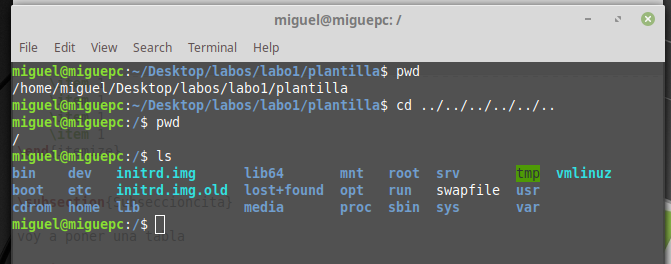
\includegraphics[width=0.5\textwidth]{img/1.png}
\caption{comandos de enunciado del 1 al 4}
\end{figure}

\begin{figure}[H]
\centering
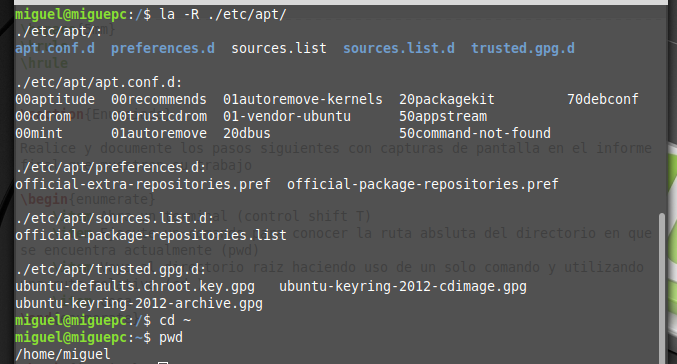
\includegraphics[width=0.5\textwidth]{img/2.png}
\caption{comandos de enunciado del 5 al 6}
\end{figure}

\begin{figure}[H]
\centering
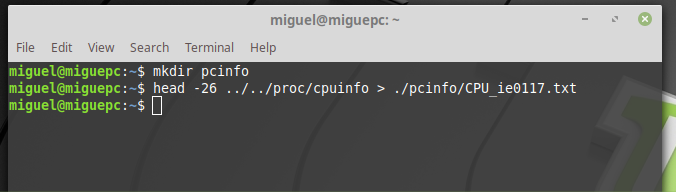
\includegraphics[width=0.5\textwidth]{img/3.png}
\caption{comandos de enunciado del 7 y 8}
\end{figure}

\begin{figure}[H]
\centering
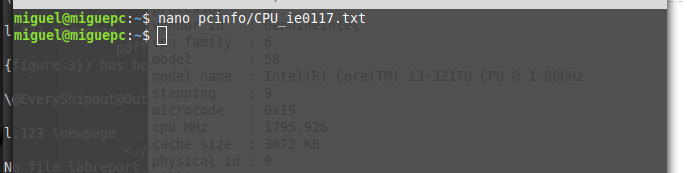
\includegraphics[width=0.5\textwidth]{img/4.png}
\caption{comandos de enunciado del 9 y 10}
\end{figure}

\begin{figure}[H]
\centering
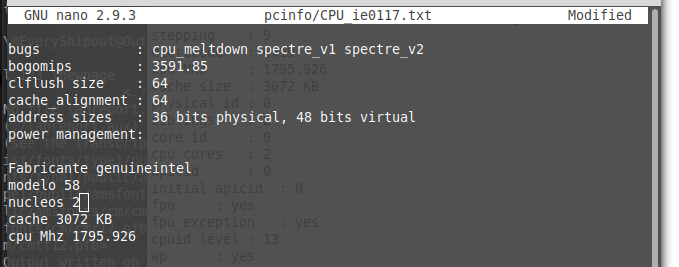
\includegraphics[width=0.5\textwidth]{img/5.png}
\caption{archivo CPU\_ie0117.txt modificado}
\end{figure}

\begin{figure}[H]
\centering
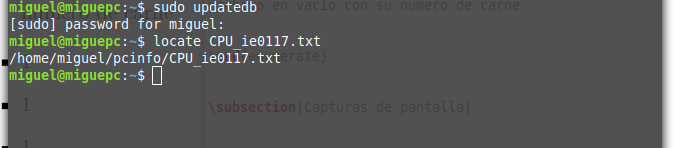
\includegraphics[width=0.5\textwidth]{img/6.png}
\caption{comandos de enunciado del 11 y 12}
\end{figure}

\begin{figure}[H]
\centering
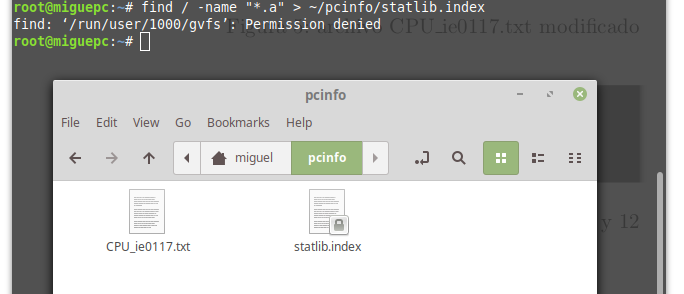
\includegraphics[width=0.5\textwidth]{img/7.png}
\caption{comandos de enunciado del 13}
\end{figure}

\begin{figure}[H]
\centering
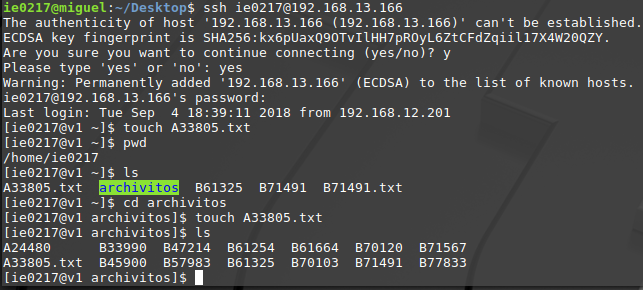
\includegraphics[width=0.5\textwidth]{img/8.png}
\caption{comandos de enunciado del 14}
\end{figure}


\newpage
\bibliographystyle{plain}
\bibliography{2.bibliography}


\end{document}
